    
\chapter{擬声語 擬音語}

\begin{center}
\begin{Large}
第157課: 擬声語: 擬音語: Animal Sounds 
\end{Large}
\end{center}
 
\par{ Everyone likes animals. Haven't you seen some today at work or school? Jokes aside, languages are not in agreement about what animals sound like. Sometimes they may sound similar across unrelated languages, but usually they don't. }

\par{\textbf{Curriculum Note }: This lesson is currently a stub lesson and will be expanded over time. }
      
\section{Animal Sounds}
 
\par{ The following table lists the most important animal sounds in Japanese. See how different they are? }

\begin{ltabulary}{|P|P|P|P|P|P|}
\hline 

Dog & ワンワン・キャンキャン & Cat & ニャーニャー & Cow & モーモー \\ \cline{1-6}

Mouse & チューチュー & Pig & ブーブー & Bee & ブンブン \\ \cline{1-6}

Chicken & コケコッコー & Horse & ヒヒーン & Frog & ケロケロ・ゲロゲロ \\ \cline{1-6}

Duck & ガーガー & Owl & ホーホー & Monster\slash lion & ガオー \\ \cline{1-6}

Sheep\slash goat & メーメー & Crow & カーカー & Bird & チッチッ \\ \cline{1-6}

Fox & コンコン & Dove & ポッポ & Cricket & コロコロ \\ \cline{1-6}

Pheasant & ケンケン & Sparrow & チュンチュン & Chick & ピヨピヨ \\ \cline{1-6}

\end{ltabulary}

\begin{center}
 \textbf{More Birds }
\end{center}

\par{ The most abundant source of animal sounds in Japanese are from birds. This is because each bird species have particular songs. As there are many indigenous bird species in Japan, pictures will be used to show you what these birds look like. }

\begin{ltabulary}{|P|P|}
\hline 

 
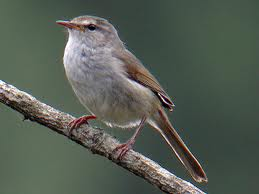
\includegraphics[scale=0.2]{figs/第04章/第157課:_onomatopoeiaii_fig/uguisu.png}
  ウグイス:ホーホケキョ 
&  
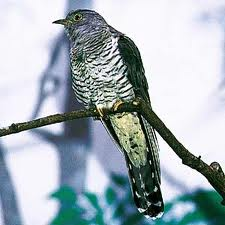
\includegraphics[scale=0.2]{figs/第04章/第157課:_onomatopoeiaii_fig/kakkoo.png}
 カッコウ:カッコー 
\\ \cline{1-2}

 
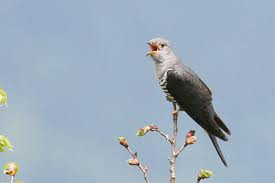
\includegraphics[scale=0.2]{figs/第04章/第157課:_onomatopoeiaii_fig/hototogisu.png}
 ホトトギス:テッペンカケタカ 
&  
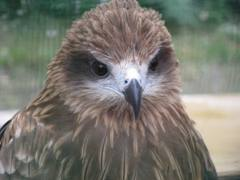
\includegraphics[scale=0.2]{figs/第04章/第157課:_onomatopoeiaii_fig/tonbi.png}
  トンビ:ピーヒョロロ 
\\ \cline{1-2}

\end{ltabulary}
\hfill\break
    